\subsection{First Order Differential Equations}
These are differential equations of the form $F(x,y,y')=0$
\subsubsection{Integrals as Solutions}
These are differential equations of the form $y'=f(x)$ or $y'=f(y)$\\
\begin{align*}
    \text{Ex: }&y'=\cos x\\
    &y=\int\cos xdx=\sin x+C
\end{align*}
\begin{align*}
    \text{Ex2: }&y'=e^{2y}\\
    &y'=\frac{dy}{dx}=\frac{1}{dx/dy}\\
    &\frac{1}{y'}=\frac{1}{dy/dx}=x'=e{-2y}\\
    &x(y)=\int e^{-2y}=-2x+C\\
    &y=-\frac{1}{2}\ln(-2x+C)
\end{align*}
\subsubsection{Slope Fields and Unique Existence}
A slope field is a vector field of equation $\brangle{1,y'}$.\\
A direction field is essentially the same thing but normalized: $\dfrac{\brangle{1,y'}}{\sqrt{1+(y')^2}}$
If function is in terms of $x$ only then plot along lines on the x-axis.\\
If the function is in terms of $y$ only then plot along lines on the y-axis.\\
\\
Existence and Uniqueness\\
If $f(x,y)$ and $\dfrac{\partial f}{\partial y}$ exists and is continuous near a point $(x_0,y_0)$ then the ODE $y'=f(x,y),\,y(x_0)=y_0$ has a solution locally and is unique.\\
A solution is considered unique if it has initial conditions such that it has only one solution.\\
\\
Ex: For what range of values does $(x-2)y''+y'+(x-2)\tan(x)y=0$ have a unique solution?
\begin{align*}
    &(x-2)y''+y'+(x-2)\tan(x)y=0\\
    &y''+\frac{1}{x-2}y'+\tan(x)y=0\text{ such that }x\neq 2\wedge x\neq \frac{\pi}{2}+n\pi,\ n\in\Z\\
    &y(3)=0,\ y'(3)=1\\
    &\therefore\text{the ODE will only have a unique solution in the continuous subdomain containing }x=3\\
    &\therefore\text{the longest interval for a unique solution is }x\in\brround{2,\frac{3\pi}{2}}
\end{align*}
\subsubsection{Separable Equations}
These are of the form $y'=f(x)g(y)$ and have solution
$$\int\frac{dy}{g(y)}=\int f(x)dx$$
\begin{align*}
    \text{Ex: }&\frac{dy}{dx}=\frac{4x}{1-y},\,y(3)=0\\
    &\int(1-y)dy=\int 4xdx\Ra y-\frac{y^2}{2}=2x^2+C\\
    &y(3)=0\Ra0=18+C\Ra C=-18\\
    &y^2-2y=36-4x^2\\
    &y^2-2y+1-1=36-4x^2\\
    &(y-1)^2=37-4x^2\\
    &y-1=\pm\sqrt{37-4x^2}\\
    &y=1\pm\sqrt{37-4x^2}\\
    &y(3)=0\therefore\,y=1-\sqrt{37-4x^2}
\end{align*}
Ex2:
\begin{align*}
    &x\frac{dy}{dx}=y\ln y\\
    &\int\frac{dy}{y\ln y}=\int\frac{dx}{x}\\
    &u=\ln y\Ra du=\frac{dy}{y}\\
    &\int\frac{dy}{y\ln y}=\int\frac{du}{u}=\ln|u|=\ln|\ln|y||\\
    &\ln|\ln|y||=\ln |x|+C\\
    &\ln|y|=Cx\\
    &y=e^{Cx}
\end{align*}
\subsubsection{Linear Differential Equations}
These are of the form $y'+p(x)y=g(x)$\\
For where $p(x)=0$, we get $y'=g(x)$ which we can solve. We can get to this point by introducing an integrating factor $r(x)$ such that
\begin{align*}
    &r(x)(y'+p(x)y)=(r(x)y)'\\
    &ry'+rpy=ry'+r'y\\
    &rp=r'
\end{align*}
We can solve to find
$$r(x)=e^{\int^xp(t)dt}$$
\begin{align*}
    \text{Ex: }&ty'+5y=24t^3,\,y(1)=2\\
    &y'=\frac{5}{t}y=24t^2\\
    &p(t)=\frac{5}{t},\,g(t)=24t^2\\
    &r(t)=e^{\int^t\frac{5ds}{s}}=e^{5\ln|t|}=t^5\\
    &(t^5y)'=t^5\brround{y'(t)+\frac{5}{t}y},\,y'+\frac{5}{t}=24t^2\\
    &(t^5y)'=t^5(24t^2)=24t^7\\
    &t^5y=\int^t24s^7ds=3t^8+C\\
    &y(1)=2,\,2=3+C\Ra C=-1\\
    &y(t)=3t^3-\frac{1}{t^5}
\end{align*}
Ex2:
\begin{align*}
    &(1+x^2)y'+2xy=\cot x\\
    &y'+\frac{2x}{1+x^2}y=\frac{\cot x}{1+x^2}\\
    &r=e^{\int pdx}=e^{\int\brround{\frac{2x}{1+x^2}}dx}=e^{\ln|1+x^2|}=1+x^2\\
    &(ry)'=rg\\
    &y=r^{-1}\int rg dx\\
    &y=\frac{1}{1+x^2}\int(1+x^2)\frac{\cot x}{1+x^2}dx=\frac{1}{1+x^2}\int\cot x dx\\
    &y=\frac{1}{1+x^2}(\ln|\sin x|+C)
\end{align*}
\subsubsection{Exact Differential Equations}
An equation in the form $M(x,y)+N(x,y)y'=0$ is exact if $M_y=N_x$.\\
We can solve an exact equation by taking the integral of $M$ or $N$ and then solving for the constants.
\begin{align*}
    \text{i.e. }&\int M dx=\phi(x,y)+h(y)\\
    &\frac{\partial}{\partial y}(\phi(x,y)+h(y))=N\\
    &\text{solve for $h(y)$ and then $\phi(x,y)+h(y)$ will be the solution}
\end{align*}
\begin{align*}
    \text{Ex: }&2x+y^2+2xyy'=0\\
    &M=2x+y^2,\ N=2xy\\
    &M_y=2y,\ N_x=2y\\
    &M_y=N_x\therefore\text{exact}\\
    &\int(2x+y^2)dx=x^2+xy^2+h(y)\\
    &\frac{\partial}{\partial y}\brround{x^2+xy^2+h(y)}=2xy+h'(y)\Ra h'(y)=0\\
    &\Ra h(y)=C\\
    &\therefore x^2+xy^2=C
\end{align*}
If an equation is not in exact form, we can sometimes multiply the equation by an integrating factor, $u$ where $u=u(x)$ or $u=u(y)$, to put it in the form of an exact equation.\\
$uM+uNy'=0$ such that $(uM)_y=(uN)_x$
\begin{align*}
    \text{Ex: }&(x+2)\sin y+(x\cos y)y'=0,\,y(1)=\frac{\pi}{2}\\
    &M=(x+2)\sin y,\ N=(x\cos y)\\
    &M_y=(x+2)\cos y,\ N_x=\cos y\\
    &M_y\neq N_x\therefore \text{ not exact}\\
    &(uM)_y=(uN)_x\\
    &\text{let }u=u(x)\\
    &uN_x+Nu'=uM_y\\
    &u\cos y+(x\cos y)u'=u(x+2)\cos y\\
    &u+xu'=u(x+2)\\
    &xu'=u(x+1)\\
    &\int\frac{du}{u}=\int\brround{1+\frac{1}{x}}dx\\
    &\ln|u|=x+\ln|x|\\
    &|u|=e^{x+\ln|x|}=|x|e^x\\
    &\text{Integrating factor: }u=xe^x\\
    &\text{set up new DE }(x+2)xe^x\sin y+(x^2e^x\cos y)y'=0,\ y(1)=\frac{\pi}{2}\\
    &M=(x+2)xe^x\sin y,\ N=(x^2e^x\cos y)\\
    &M_y=(x^2e^x+2xe^x)\cos y=N_x\therefore \text{ exact}\\
    &\int(x^2e^x\cos y)dy=x^2e^x\sin y+h(x)\\
    &\frac{\partial}{\partial x}(x^2e^x\sin y+h(x))=x^2e^x\sin y+2xe^x\sin y+h'(x)=(x^2e^x\sin y+2xe^x\sin y)\Ra h'(x)=0\\
    &\Ra h(x)=C\\
    &x^2e^x\sin y=C\\
    &y(1)=\frac{\pi}{2}\Ra e=C\\
    &\therefore x^2e^x\sin y=e
\end{align*}
\subsubsection{Autonomous Differential Equations}
This involves finding the properties of solutions of DEs without actually solving them.\\
If $\lim\limits_{x\to\infty}y'=0$ then the function will attain a constant value. For the case where $y'=y'(y)$ then we can analyze how specific values of $y(0)$ will behave as the function approaches infinity.\\
Definitions:
\begin{itemize}
    \item If the value of a function at infinity does not change, it is a \textit{fixed point}.
    \item If the function converges to a fixed point from both sides, it is said to be \textit{asymptotically stable}.
    \item If the function diverges from a fixed point on either side, it is said to be \textit{unstable}.
    \item If a function converges to a fixed point from only one side, it is said to be \textit{metastable} or \textit{semistable}.
\end{itemize}
Phase line diagrams:\\
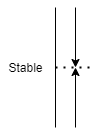
\includegraphics[scale=1]{Images/ODEPictures/PhaseLineStable.png} 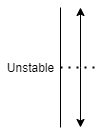
\includegraphics[scale=1]{Images/ODEPictures/PhaseLineUnstable.png}
\subsubsection{Numerical Methods}
These are methods used to approximate solutions.\\
One such method is Euler's Method which states that we can express the line $y=y(t)$ as a collection of tiny line segments.\\
We can express $y'=f(t,y)$ and $y(t_0)=y_0$ on the range from $t_0$ to $T$. In this range, we will have $N$ intervals of width $h=\Delta t=\frac{T-t_0}{N}$ where $t_k=t_0+kh$. This gives us
$$y(t)=\eqnsystem{y_1=y_0+f(t_0,y_0),\ t\geq t_0\\
y_2=y_1+f(t_1,y_1),\ t_0\leq t< t_1\\
y_3=y_2+f(t_2,y_2),\ t_1\leq t<t_2\\
\vdots\\
y_k=y_{k-1}+f(t_{k-1},y_{k-1}),\ t_{k-1}\leq t<t_k}$$
The error is approximately $E\approx Ch$ for some $h$.\\
\\
Improved Euler's Method:
\begin{align*}
    &k_1=f(t_n,y_n)\\
    &k_2=f(t_n+h,y_n+hk_1)\\
    &y_{n+1}=y_n+\frac{h}{2}(k_1+k_2)
\end{align*}
Error is approximately $E\approx Ch^2$\\
\\
Range-Kutta Method:
\begin{align*}
    &k_1=f(t_n,y_n)\\
    &k_2=f\brround{t_n+\frac{h}{2},y_n+h\frac{k_1}{2}}\\
    &k_3=f\brround{t_n+\frac{h}{2},y_n+h\frac{k_2}{2}}\\
    &k_4=f(t_n+h,y_n+hk_3)\\
    &y_{n+1}=y_n+\frac{h}{6}(k_1+2k_2+2k_3+k_4)
\end{align*}